\section{Chainsewing Attack Simulation}
\label{sec:simulation}

To measure the success rate of the chainsewing attack against the na\"ive NIPoPoW construction described in Section~\ref{sec:attack}, we implemented a simulation to estimate the probability of the adversary generating a winning NIPoPoW against the honest party\footnote{\ifanonymous{A link to the open source implementation of the attack simulation has been removed for anonymization purposes}\else{The simulation implementation is available for reproduction purposes under an MIT license at \url{https://github.com/decrypto-org/nipopow-velvet/tree/master/chainsew}}\fi}. Our experimental setting is as follows. We fix $\mu_A = 0$ (in case the verifier checks previd pointer consistency, we can set $\mu_A = 1$) and $\mu_B = 10$ as well as the required length of the suffix $k = 15$. We fix the adversarial mining power to $t = 1$ and $n = 5$ which gives a $20\%$ adversary. We then vary the NIPoPoW security parameter for the $\pi$ portion from $m = 3$ to $m = 30$. We then run $100$ Monte Carlo simulations and measure whether the adversary was successful in generating a competing NIPoPoW which compares favourably against the adversarial NIPoPoW.

\begin{figure}
	\begin{center}
		\iftwocolumn
			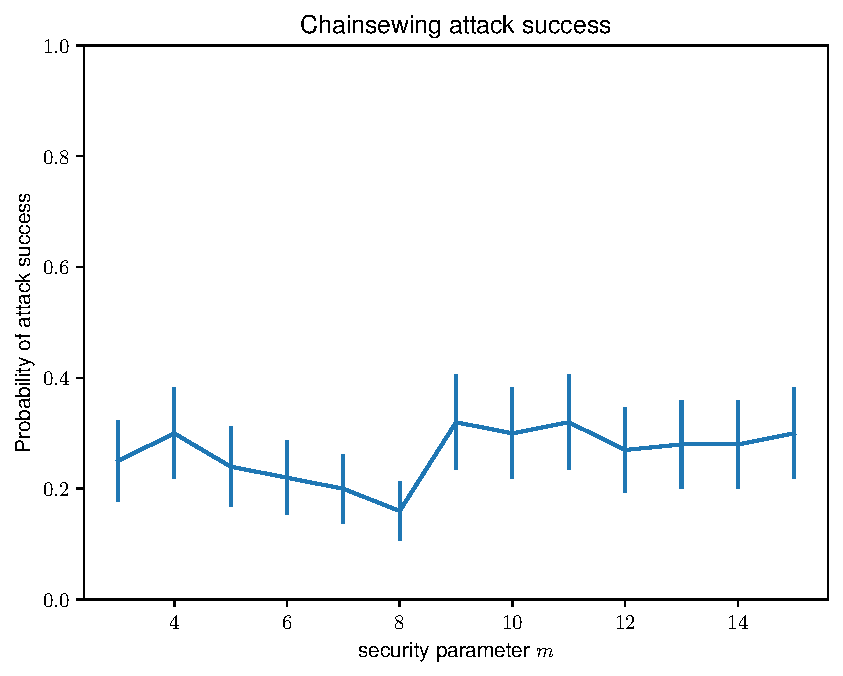
\includegraphics[width=0.9\columnwidth]{figures/attack-confidence.pdf}
		\else
			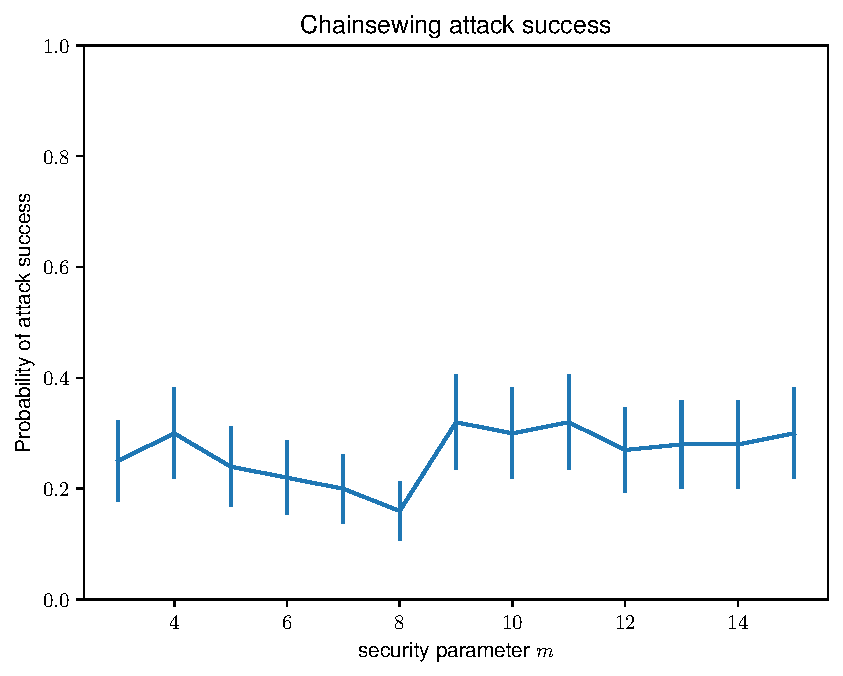
\includegraphics[width=0.7 \columnwidth]{figures/attack-confidence.pdf}
		\fi
	\end{center}
	\caption{The measured probability of success of the Chainsewing attack mounted under our parameters for varying values of the security parameter $m$. Confidence intervals at $95\%$.}
	\label{fig:confidence}
\end{figure}

For performance reasons, our model for the simulation slightly deviates from the Backbone model on which the theoretical analysis of Section~\ref{sec:analysis} is based and instead follows the simpler model of Ren~\cite{nakamoto-simple}. This model favours the honest parties, and so provides a lower bound for probability of adversarial success, which implies that our attack efficacy is in reality better than estimated here. In this model, block arrival is modelled as a Poisson process and blocks are deemed to belong to the adversary with probability $t / n$, while they are deemed to belong to the honest parties with probability $(n - t) / n$. Block propagation is assumed instant and every party learns about a block as soon as it is mined. As such, the honest parties are assumed to work on one common chain and the problem of non-uniquely successful rounds does not occur.

We consistently find a success rate of approximately $0.26$ which remains more or less constant independent of the security parameter, as expected. We plot our results with $95\%$ confidence intervals in Figure~\ref{fig:confidence}. This is in contrast with the best previously known attack in which, for all examined values of the security parameter, the probability of success remains below $1\%$.
